\documentclass[a4paper,12pt]{article}
\usepackage[utf8]{inputenc}
\usepackage[spanish]{babel}
\usepackage{color}
\usepackage{parskip}
\usepackage{graphicx}
\usepackage{multirow}
\usepackage{listings}
\usepackage{vmargin}
\graphicspath{ {imagenes/} }
\definecolor{mygreen}{rgb}{0,0.6,0}
\definecolor{lbcolor}{rgb}{0.9,0.9,0.9}
\usepackage{epstopdf}


\setpapersize{A4}
\setmargins{2.5cm}       % margen izquierdo
{1.5cm}                        % margen superior
{16.5cm}                      % anchura del texto
{23.42cm}                    % altura del texto
{10pt}                           % altura de los encabezados
{1cm}                           % espacio entre el texto y los encabezados
{0pt}                             % altura del pie de página
{2cm}     

\lstset{
backgroundcolor=\color{lbcolor},
    tabsize=4,    
%   rulecolor=,
    language=SQL,
        basicstyle=\tiny,
        aboveskip={1.5\baselineskip},
        columns=fixed,
        showstringspaces=false,
        extendedchars=false,
        breaklines=true,
        prebreak = \raisebox{0ex}[0ex][0ex]{\ensuremath{\hookleftarrow}},
        frame=single,
        showtabs=false,
        showspaces=false,
        showstringspaces=false,
        identifierstyle=\ttfamily,
        keywordstyle=\color[rgb]{0,0,1},
        commentstyle=\color[rgb]{0.026,0.112,0.095},
        stringstyle=\color{red},
        numberstyle=\color[rgb]{0.205, 0.142, 0.73},
%        \lstdefinestyle{C++}{language=C++,style=numbers}’.
}
\begin{document}


\twocolumn[\section{Códigos}]
\subsection{Código usado para crear las tablas}

\lstinputlisting{sesion3.sql}
\break

\subsection{Código usado para insertar datos}

\lstinputlisting{sesion3Inserts.sql}

\onecolumn

\twocolumn[\section{Visualización en los diferentes gestores}]

\subsection{SQL Server}

\begin{figure}[h]
\centering
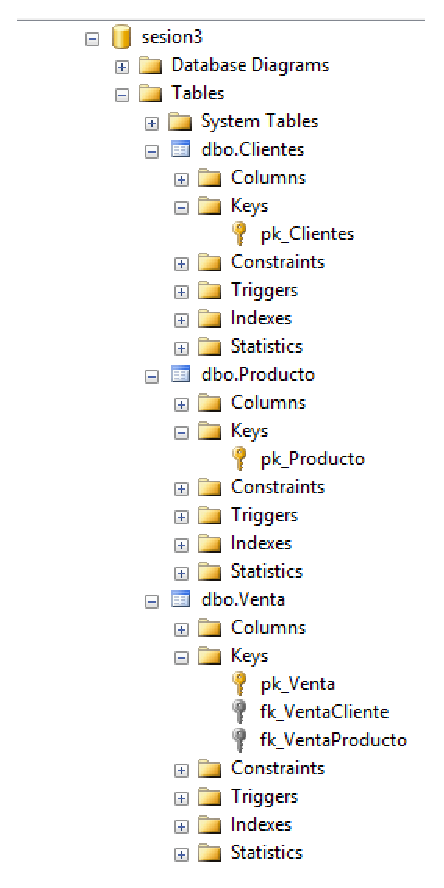
\includegraphics[scale=0.5]{1.eps}
\caption{Estructura en SQL Server}
\end{figure}

\subsection{PostgreSQL}

\begin{figure}[h]
\centering
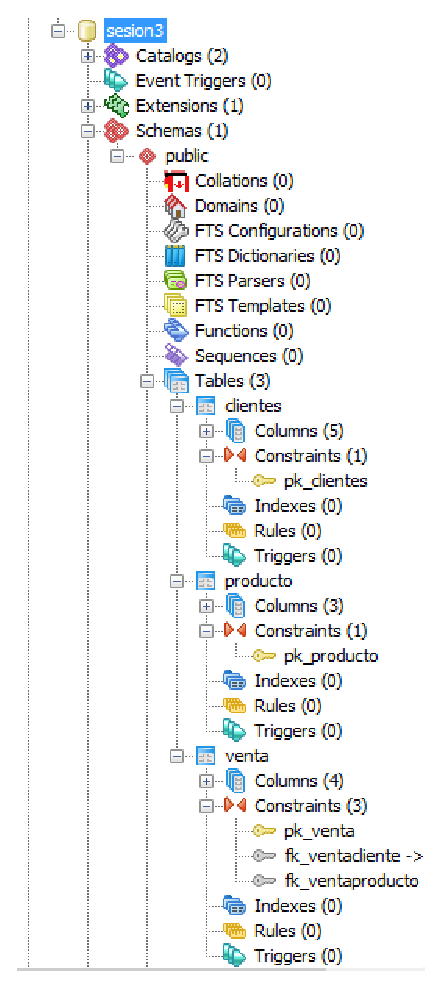
\includegraphics[scale=0.42]{2.eps}
\caption{Estructura en PostgreSQL}
\end{figure}

\break

\subsection{MySQL}

\begin{figure}[h]
\centering
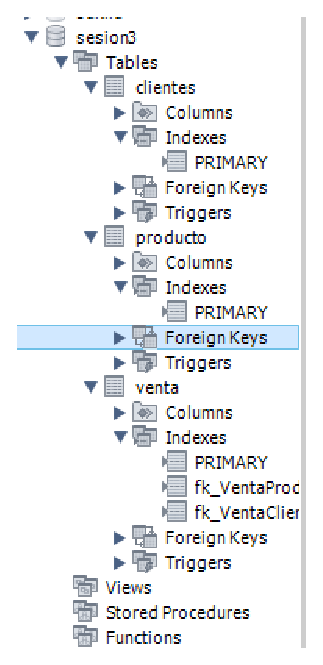
\includegraphics[scale=0.5]{3.eps}
\caption{Estructura en MySQL}
\end{figure}

\end{document}
